\documentclass[handout]{beamer}
\usepackage[utf8]{inputenc}
\usepackage[T1]{fontenc}
\usepackage{url}
\usepackage{hyperref}
\usepackage{xcolor}
\usepackage{appendixnumberbeamer}
\usepackage{amsmath}
\usepackage{bm}
\usetheme[sectionpage=progressbar,
          subsectionpage=progressbar,
          numbering=fraction,
          progressbar=none,
          background=light]{metropolis}
\usefonttheme[onlymath]{serif}

\title{From PCA to Autoencoders}
\subtitle{Unsupervised Representation Learning}
\date{December 17, 2019}
\author{\textsc{Florent Forest}\\
\scriptsize{PhD student in Data science \& Machine learning\\
Safran Aircraft Engines --- Université Paris 13}
\vspace{0.2cm}\\
\includegraphics[height=0.35cm]{./rc/e-mail-envelope-blue}\;\scriptsize{\href{mailto:forest@lipn.univ-paris13.fr}{forest@lipn.univ-paris13.fr}}\\
\includegraphics[height=0.35cm]{./rc/grid-world-blue}\;\scriptsize{\href{http://florentfo.rest}{http://florentfo.rest}}\\
\includegraphics[height=0.35cm]{./rc/github-logo-blue}\;\scriptsize{\href{https://github.com/FlorentF9}{FlorentF9}}\\
}
\institute{\vfill\hfill
\includegraphics[height=1.75cm]{./rc/logo_supaero}}

\begin{document}

  \maketitle

  \begin{frame}{Table of contents}
    \setbeamertemplate{section in toc}[sections numbered]
    \begin{small}
      \vspace{0.5cm}
      \tableofcontents%[hideallsubsections]
    \end{small}
  \end{frame}

  %%%
  \section{Introduction to autoencoders}
  %%%

  %
  \subsection{Motivations}
  %

  \begin{frame}{Motivations}

    \begin{block}{Where we are}
      \begin{itemize}
        \item Complex and high-dimensional data (i.e. $d \sim [10^3, 10^6[$)
        \item "Big Data" (i.e. $N \sim [10^5, 10^9[$)
        \item No labels (unsupervised learning)
      \end{itemize}
    \end{block}
    \pause
    \begin{block}{What we have seen so far}
      \begin{itemize}
        \item Linear dimensionality reduction techniques (e.g. PCA)\\
        $\rightarrow$ cannot learn complex transformations
        \item Non-linear techniques, e.g. t-SNE\\
        $\rightarrow$ not scalable, time complexity is $\mathcal{O}(d \cdot N^2)$, or $\mathcal{O}(d \cdot N\log N)$ with Barnes-Hut (but limited to output dimension $\leq 3$)
      \end{itemize}
    \end{block}

  \end{frame}

  \begin{frame}{Motivations}
    
    \metroset{block=fill}

    \begin{block}{So why not use (deep) neural networks?}
      \begin{itemize}
        \item Can learn complex transformations
        \item Comfortable in very-high-dimensional spaces
        \item Scale linearly with the size of data
      \end{itemize}
    \end{block}
    
  \end{frame}

  %
  \subsection{Definition}
  %

  \begin{frame}{Definition}

    \metroset{block=fill}

    \begin{exampleblock}{Definition}
      \small{
      An \alert{autoencoder} is a neural network trained to \textbf{reconstruct its inputs}. It is composed of two components:
      \vspace{-0.4cm}
      \begin{enumerate}
        \item an \alert{encoder}, mapping the input to a latent representation ("code") $\mathbf{z} = \mathbf{f}_{\boldsymbol{\phi}}(\mathbf{x})$
        \item a \alert{decoder}, mapping the code back to the input space $\tilde{\mathbf{x}} = \mathbf{g}_{\boldsymbol{\theta}}(\mathbf{z})$
      \end{enumerate}
      }
    \end{exampleblock}
    \vspace{-0.25cm}
    \begin{figure}
      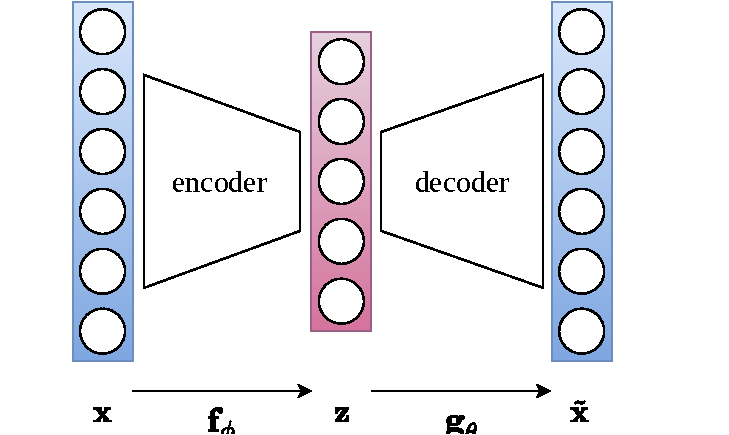
\includegraphics[height=4.5cm]{rc/autoencoder}
    \end{figure}

  \end{frame}

  \begin{frame}{Definition}

    \metroset{block=fill}

    \begin{alertblock}{Challenge}
      We do not want the encoder to learn the identity function, but to learn a \emph{good representation} of our data.
    \end{alertblock}

    \vspace{0.5cm}
    \pause

    \begin{block}{Regularization?}<2->
      Reducing the size of the \emph{hypothesis set} $\mathcal{H}$ by constraining the space of possible solutions to the optimization problem.
      \vspace{-0.25cm}
      \begin{itemize}
        \item L2 weight decay
        \item Sparsity, L1 weight decay
        \item \dots
      \end{itemize}
    \end{block}
    
  \end{frame}

  %
  \subsection{Mathematical formulation}
  %

  \begin{frame}{What is a good representation?}

    \metroset{block=fill}
    
    \small{Let $q_{\boldsymbol{\phi}}(Z|X)$ be a (stochastic) parametric mapping from $X$ to $Z$. A good representation $Z$ of a random variable $X$ maximizes \alert{mutual information} between $X$ and $Z$ (\emph{infomax principle}):}
    \vspace{0cm}
    \begin{align*}
      \mathbb{I}(X;Z) &= \mathbb{H}(X) - \mathbb{H}(X|Z)\\
                      &= C(X) + \mathbb{E}_{q_{\boldsymbol{\phi}}(X,Z)}\left[\log q_{\boldsymbol{\phi}}(X|Z)\right]
    \end{align*}
    \pause
    \small{For any parametric distribution $p_{\boldsymbol{\theta}}(X|Z)$ we have $\mathbb{E}_{q_{\boldsymbol{\phi}}(X,Z)}\left[\log p_{\boldsymbol{\theta}}(X|Z)\right] \leq \mathbb{E}_{q_{\boldsymbol{\phi}}(X,Z)}\left[\log q_{\boldsymbol{\phi}}(X|Z)\right]$ (using $D_{KL}(q||p) \geq 0$).}
    \pause
    \vspace{0.5cm}
    \begin{block}{Task: maximize a lower bound on $\mathbb{I}(X;Z)$}
      \begin{equation*}
        \underset{\boldsymbol{\phi},\boldsymbol{\theta}}{\text{maximize}} \; \mathbb{E}_{q_{\boldsymbol{\phi}}(X,Z)}\left[\log p_{\boldsymbol{\theta}}(X|Z)\right]
      \end{equation*}
    \end{block}

  \end{frame}

  \begin{frame}{Loss function for deterministic autoencoders}

    We consider \alert{deterministic} mappings $Z = \mathbf{f}_{\boldsymbol{\phi}}(X)$ (i.e. $q_{\boldsymbol{\phi}}(Z|X) = \delta(Z - \mathbf{f}_{\boldsymbol{\phi}}(X))$) and $\tilde{X} = \mathbf{g}_{\boldsymbol{\theta}}(\mathbf{f}_{\boldsymbol{\phi}}(X))$.
    \vspace{0cm}
    \begin{equation*}
      \underset{\boldsymbol{\phi},\boldsymbol{\theta}}{\text{maximize}} \; \mathbb{E}_{q_{\boldsymbol{\phi}}(X)}\left[\log p_{\boldsymbol{\theta}}(X|Z = \mathbf{f}_{\boldsymbol{\phi}}(X))\right]
    \end{equation*}
    \pause
    Using empirical mean over a set of data samples:
    \vspace{0cm}
    \begin{equation*}
      \underset{\boldsymbol{\phi},\boldsymbol{\theta}}{\text{maximize}} \; \sum_i \log p_{\boldsymbol{\theta}}(\mathbf{x}^{(i)}|\mathbf{z}^{(i)} = \mathbf{f}_{\boldsymbol{\phi}}(\mathbf{x}^{(i)}))
    \end{equation*}

    equivalent to:
    \vspace{0cm}
    \begin{equation*}
      \underset{\boldsymbol{\phi},\boldsymbol{\theta}}{\text{maximize}} \; \sum_i \log p(\mathbf{x}^{(i)}|\tilde{\mathbf{x}}^{(i)} = \mathbf{g}_{\boldsymbol{\theta}}(\mathbf{f}_{\boldsymbol{\phi}}(\mathbf{x}^{(i)})))
    \end{equation*}
    \pause
    Let us turn this into a minimization of the negative sum of individual loss functions $\mathcal{L}(\mathbf{x}, \tilde{\mathbf{x}}) = -\log p(\mathbf{x}|\tilde{\mathbf{x}})$.
    
  \end{frame}

  \begin{frame}{Loss function for deterministic autoencoders}

    \metroset{block=fill}

    The reconstruction $\tilde{\mathbf{x}}$ is the \alert{mean} of a distribution that may have generated $\mathbf{x}$.
    \pause
    \begin{block}{Continuous variables: $\mathbf{x} \in \mathbb{R}^d$}
      \begin{itemize}
        \item Gaussian distribution: $X|\tilde{X} = \tilde{\mathbf{x}} \sim \mathcal{N}(\tilde{\mathbf{x}}, \mathbf{\sigma}^2 \mathbf{I})$
      \item Loss function: $\mathcal{L}(\mathbf{x}, \tilde{\mathbf{x}}) \propto ||\mathbf{x} - \tilde{\mathbf{x}}||_2^2$
      \end{itemize}
      $\rightarrow$ \alert{Mean Squared Error (MSE) loss}
    \end{block}
    \pause
    \begin{block}{Binary variables: $\mathbf{x} \in \{0,1\}^d$, or $\mathbf{x} \in [0,1]^d$}
      \begin{itemize}
        \item Bernoulli distribution: $X|\tilde{X} = \tilde{\mathbf{x}} \sim \mathcal{B}(\tilde{\mathbf{x}})$
        \item Loss function: $-\sum_{j=1}^d [\mathbf{x}_j \log \tilde{\mathbf{x}}_j + (1-\mathbf{x}_j) \log (1-\tilde{\mathbf{x}}_j)]$
      \end{itemize}
      $\rightarrow$ \alert{Cross-entropy loss}
    \end{block}
    
  \end{frame}

  %%%
  \section{Links with Principal Component Analysis (PCA)}
  %%%

  %
  \subsection{Can neurons learn principal components?}
  %

  \begin{frame}{Hebb's learning rule}

    \begin{columns}[T,onlytextwidth]
      \column{0.7\textwidth}
      \vspace{0.5cm}
      Back to 1949 $\rightarrow$ Hebbian learning
      \column{0.3\textwidth}
      \includegraphics[height=1.5cm]{rc/delorean}
    \end{columns}
    \pause
    \metroset{block=fill}

    \begin{block}{The artificial neuron and Hebb's learning rule \cite{hebb-organization-of-behavior-1949}}
      \begin{columns}[T,onlytextwidth]
        \column{0.6\textwidth}
        \vspace{0.7cm}
        \centering
        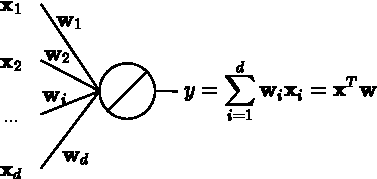
\includegraphics[]{rc/artificial-neuron}

        \column{0.4\textwidth}
        \vspace{0.7cm}
        \centering
        \small{Weights increase if input and output are correlated.}
        \begin{equation*}
          \Delta \mathbf{w}_i = \alpha \mathbf{x}_i y
        \end{equation*}
        \begin{equation*}
          \Delta \mathbf{w} = \alpha \mathbf{x} y = \alpha \mathbf{x} \mathbf{x}^T \mathbf{w}
        \end{equation*}
      \end{columns}
    \end{block}
    
    See for example Rosenblatt's \textbf{perceptron} (1958) \cite{Rosenblatt58theperceptron} for an illustration of this learning rule.

  \end{frame}

  \begin{frame}{Learning principal components with Oja's rule}

    \textbf{Problem:} the weights can "explode" with Hebb's rule. A solution is to add a \emph{forgetting term}.
    \pause
    \metroset{block=fill}

    \begin{block}{Oja's learning rule \cite{Oja1982}}
      \begin{equation*}
        \Delta \mathbf{w} = \alpha (\mathbf{x} y - y^2 \mathbf{w})
      \end{equation*}
    \end{block}
    \pause
    \scriptsize{
    We can show that this rule leads to \emph{principal components} \cite{Becker1991,Oja1992}: 
    \vspace{0cm}
    \begin{equation*}
      \Delta \mathbf{w} = \alpha (\mathbf{x} \mathbf{x}^T \mathbf{w} - \mathbf{w}^T \mathbf{x} \mathbf{x}^T \mathbf{w} \mathbf{w})
    \end{equation*}
    After convergence, we have:
    \begin{align*}
      \mathbb{E}\left[\Delta \mathbf{w}\right] = \alpha (\mathbb{E}\left[\mathbf{x} \mathbf{x}^T\right] \mathbf{w} - \mathbf{w}^T \mathbb{E}\left[\mathbf{x} \mathbf{x}^T\right] \mathbf{w} \mathbf{w}) = \alpha (\mathbf{C} \mathbf{w} - \mathbf{w}^T \mathbf{C} \mathbf{w} \mathbf{w}) = 0
    \end{align*}
    
    where $\mathbf{C} = \mathbb{E}\left[\mathbf{x} \mathbf{x}^T\right]$ is the covariance matrix. Finally:
    \vspace{0cm}
    \begin{equation*}
      \mathbf{C} \mathbf{w} = \mathbf{w}^T \mathbf{C} \mathbf{w} \mathbf{w} = \lambda \mathbf{w}
    \end{equation*}

    Thus, $\mathbf{w}$ is an eigenvector of the covariance matrix, a.k.a. a \textbf{principal component}.
    }

  \end{frame}

  %%%
  \subsection{Linear autoencoders}
  %%%

  \begin{frame}{Definition}

    \begin{figure}
      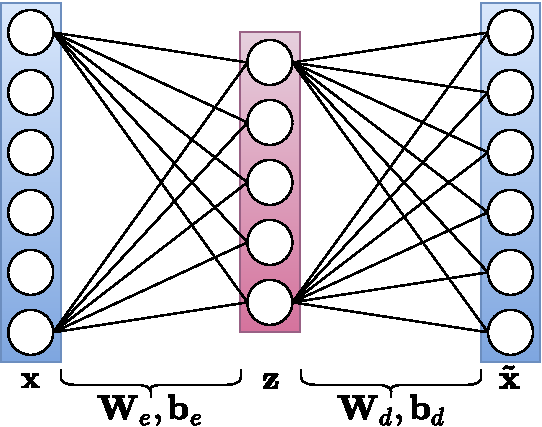
\includegraphics[width=5.5cm]{rc/linear-autoencoder}
    \end{figure}
    \vspace{-0.25cm}
    \begin{equation*}
      \tilde{\mathbf{x}} = \mathbf{W}_d \left(\mathbf{W}_e \mathbf{x} + \mathbf{b}_e\right) + \mathbf{b}_d
    \end{equation*}
    \pause
    Ignoring the biases, the MSE loss becomes:
    \vspace{0cm}
    \begin{align*}
      \text{MSE} &= \sum_i ||\mathbf{x}^{(i)} - \tilde{\mathbf{x}}^{(i)}||_2^2 = \sum_i ||\mathbf{x}^{(i)} - \mathbf{W}_d \mathbf{W}_e \mathbf{x}^{(i)}||_2^2 \\
                 &= ||\mathbf{X} - \mathbf{X} \mathbf{W}_d \mathbf{W}_e||_F^2
    \end{align*}
    
  \end{frame}

  \begin{frame}{Equivalence to PCA}

    \begin{columns}[T,onlytextwidth]
      \column{0.5\textwidth}
      \centering \textbf{PCA}
      \begin{align*}
        \underset{\mathbf{U} \in \mathbb{R}^{d \times r}}{\text{minimize}} &\; ||\mathbf{X} - \mathbf{X} \mathbf{U} \mathbf{U}^T||_F^2 \\
        \text{subject to} &\; \mathbf{U}^T \mathbf{U} = \mathbf{I}
      \end{align*}
      \pause
      \column{0.5\textwidth}
      \centering \textbf{Linear AE}
      \begin{equation*}
        \underset{\mathbf{W}_e \in \mathbb{R}^{l \times d}, \mathbf{W}_d \in \mathbb{R}^{d \times l}}{\text{minimize}} \; ||\mathbf{X} - \mathbf{X} \mathbf{W}_d \mathbf{W}_e||_F^2
      \end{equation*}
      {\scriptsize one can show that we must have $\mathbf{W}_e = \mathbf{W}_d^{\dagger}$ (pseudo-inverse), then:}
      \begin{equation*}
        \underset{\mathbf{W} \in \mathbb{R}^{d \times l}}{\text{minimize}} \; ||\mathbf{X} - \mathbf{X} \mathbf{W} \mathbf{W}^{\dagger}||_F^2
      \end{equation*}

    \end{columns}

    \vspace{1cm}
    \pause
    \centering
    $\blacktriangleright$ Linear autoencoders are equivalent to PCA\dots\\
    \alert{without the orthogonality constraint}! \cite{Plaut2018}
    
  \end{frame}

  \begin{frame}{Equivalence to PCA}

    \begin{figure}
      \includegraphics[width=\textwidth]{rc/pca-ae-bases}\\
      \tiny{\url{https://towardsdatascience.com/understanding-variational-autoencoders-vaes-f70510919f73}}
    \end{figure}
    
  \end{frame}

  %%%
  \section{Real-life autoencoders}
  %%%

  %
  \subsection{Non-linear and deep autoencoders}
  %

  \begin{frame}{Non-linear and deep autoencoders}

    \begin{figure}
      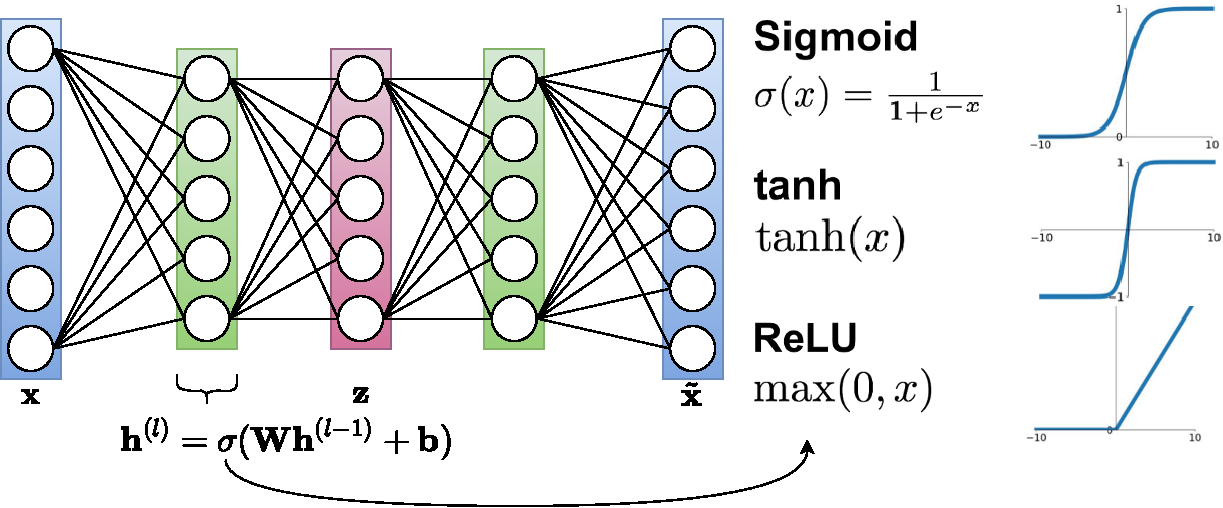
\includegraphics[width=\textwidth]{rc/deep-autoencoder}
    \end{figure}
    
    \pause
    \centering
    $\blacktriangleright$ \alert{Not equivalent to PCA!}

    \pause
    {\small Trained end-to-end with backprop and SGD. Layer-wise pre-training \cite{Hinton2006} is in fact not necessary (thanks to ReLU, better optimization, etc.).}

  \end{frame}

  %
  \subsection{Different types of regularizations}
  %

  \begin{frame}{Undercomplete or overcomplete}

    Let $d$ be the input dimension and $l$ the code dimension.
    \pause
    \vspace{0.5cm}
    \begin{columns}[T,onlytextwidth]
      \column{0.5\textwidth}
      \centering
      $l < d$: \textbf{undercomplete}
      \begin{figure}
        \includegraphics[height=3cm]{rc/entonnoirs1}
      \end{figure}
      \pause
      \column{0.5\textwidth}
      \centering
      $l \geq d$: \textbf{overcomplete}
      \begin{figure}
        \includegraphics[height=3cm]{rc/entonnoirs2}
      \end{figure}
    \end{columns}
    \vspace{0.5cm}
    \pause
    Having the autoencoder encode the data to a lower dimension (in general $l << d$), forces it to compress the data and learn an efficient representation and is a \alert{form of regularization}.
    
  \end{frame}

  \begin{frame}{Let's code! (1)}

    \centering
    \includegraphics[width=0.5\textwidth]{rc/colab}\\
    \vspace{1cm}
    \includegraphics[width=0.25\textwidth]{rc/jupyter}

    % AE classique avec une/plusieurs couches
    % Entraîner sur MNIST avec différents loss (MSE, cross-entropy)
    % Éventuellement convolutif

    % Observer l'espace latent via t-SNE (comparer avec t-SNE sur MNIST brut)
    
  \end{frame}

  \begin{frame}{The danger of overfitting}
    
    \textbf{Problems:} overcomplete AE will not learn useful representations; and even undercomplete AE with a \emph{single continuous latent variable} can remember an entire training set (one real number per sample).

    \begin{figure}
      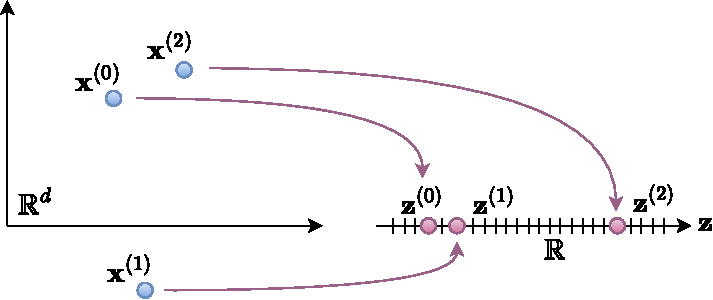
\includegraphics[width=0.8\textwidth]{rc/ae-real-numbers}
    \end{figure}
    \pause
    \textbf{Solution:} adding \alert{constraints} to the latent space by using different types of \alert{regularization}! 

  \end{frame}

  \begin{frame}{Sparse autoencoders}

    \metroset{block=fill}

    \begin{block}{Principle}
      \small{
      Sparse autoencoders can have more latent units than input units, but \alert{only a few are allowed to activate together}:
      \vspace{-0.25cm}
      \begin{itemize}
        \item a fixed proportion (e.g. 5\%) using a KL-divergence penalty \cite{Ng2011}
        \item a fixed number $k$ \cite{Makhzani2013}
        \item using a L1 penalty \cite{Arpit2016}
      \end{itemize}
      }
    \end{block}
    
    \centering
    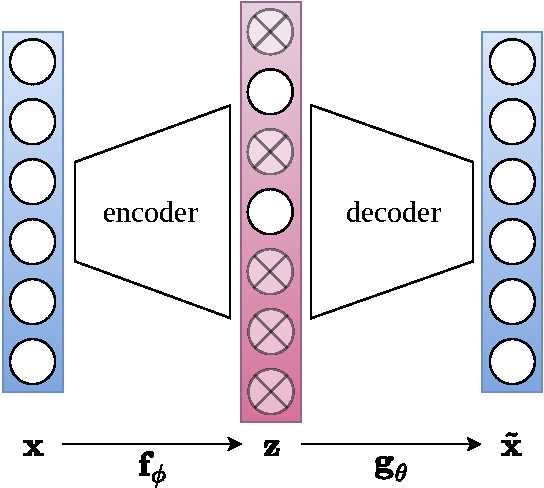
\includegraphics[width=4.5cm]{rc/sparse-autoencoder}
    
  \end{frame}

  \begin{frame}{Denoising autoencoders}

    \metroset{block=fill}

    \begin{block}{Principle}
      Denoising autoencoders \cite{Vincent2010} are trained to reconstruct \alert{corrupted} versions of the input. Corruption can be achieved by adding noise or randomly turning off input units. Usually, they have a single hidden layer with a non-linearity.
    \end{block}

    \centering
    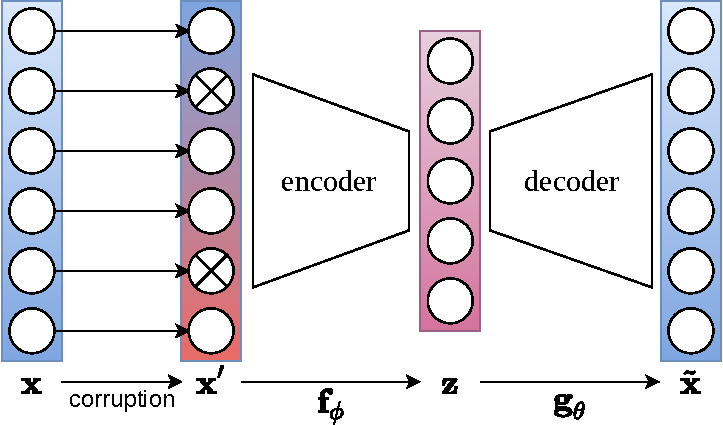
\includegraphics[width=7cm]{rc/denoising-autoencoder}
    
  \end{frame}

  %
  \subsection{Variational autoencoders (VAE)}
  %

  \begin{frame}{Motivations}
    
    \textbf{Limitation of standard AE:} the latent space has \emph{no structure} and may not be continuous; it may \emph{overfit}, and we cannot explore it nor \emph{sample} from it.
    \pause
    \begin{columns}[T,onlytextwidth]
      \column{0.5\textwidth}
      \centering
      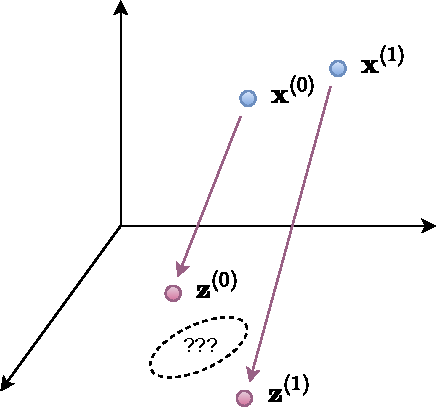
\includegraphics[width=0.8\textwidth]{rc/ae-latent}
      \pause
      \column{0.5\textwidth}
      \centering
      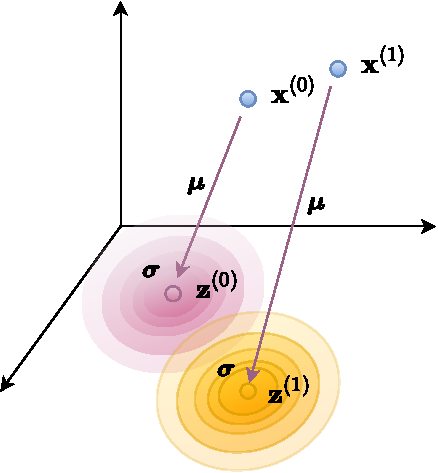
\includegraphics[width=0.8\textwidth]{rc/vae-latent}
    \end{columns}

  \end{frame}

  \begin{frame}{Motivations}

    \begin{columns}[T,onlytextwidth]
      \column{0.5\textwidth}
      \centering
      \includegraphics[height=4.25cm,width=\textwidth]{rc/vae-mnist}\\

      \column{0.4\textwidth}
      \centering
      \includegraphics[height=4.25cm,width=\textwidth]{rc/vae-faces}\\
    \end{columns}
    
    \centering
    \includegraphics[width=0.7\textwidth]{rc/vae-faces-smile}\\
    \tiny{\url{jmetzen.github.io/2015-11-27/vae.html}, \url{ermongroup.github.io/cs228-notes/extras/vae}, \url{github.com/davidsandberg/facenet}}

  \end{frame}

  \begin{frame}{Variational autoencoders (VAE)}

    \metroset{block=fill}

    VAEs are \alert{latent-variable probabilistic models}.
    \pause
    \begin{columns}[T,onlytextwidth]

      \column{0.7\textwidth}
      \begin{block}{Probabilistic setting}
        Generative model $p_{\boldsymbol{\theta}}(\mathbf{x}, \mathbf{z})$:
        \begin{enumerate}
          \item $\mathbf{z}$ is sampled from the \alert{prior} $p_{\boldsymbol{\theta}}(\mathbf{z})$
          \item $\mathbf{x}$ is generated with \alert{likelihood} $p_{\boldsymbol{\theta}}(\mathbf{x}|\mathbf{z})$ (\emph{probabilistic decoder})
        \end{enumerate}
      \end{block}

      \column{0.29\textwidth}
      \centering
      \includegraphics[width=\textwidth]{rc/vae-gen}\\
      \tiny{Kingma \& Welling 2014 \cite{Kingma2014}}
      
    \end{columns}
    \vspace{0.5cm}
    \pause
    \textbf{Problem:} $\boldsymbol{\theta}$ is a NN, so $p_{\boldsymbol{\theta}}(\mathbf{x})$ and $p_{\boldsymbol{\theta}}(\mathbf{z}|\mathbf{x})$ are intractable.\\
    \pause
    $\blacktriangleright$ Stochastic Gradient Variational Bayes (SGVB) \cite{Kingma2014} is an efficient estimation method in case of intractable marginal likelihood/posterior and large datasets.

  \end{frame}

  \begin{frame}{Variational autoencoders (VAE)}

    \begin{figure}
      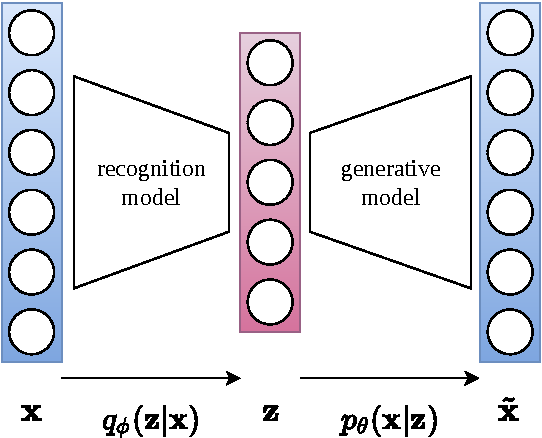
\includegraphics[width=7cm]{rc/vae}
    \end{figure}

    Recognition model $\rightarrow$ \alert{approximate posterior} $q_{\boldsymbol{\phi}}(\mathbf{z}|\mathbf{x})$\\
    (\emph{probabilistic encoder})

  \end{frame}

  \begin{frame}{VAE loss function}

    \metroset{block=fill}
    
    \begin{exampleblock}{VAE ELBO (evidence lower bound)}
      \vspace{-0.25cm}
      \begin{equation*}
        \underset{\boldsymbol{\phi},\boldsymbol{\theta}}{\text{maximize}} \; -D_{KL}\left(q_{\boldsymbol{\phi}}(Z|X)||p_{\boldsymbol{\theta}}(Z)\right) + \mathbb{E}_{q_{\boldsymbol{\phi}}(Z|X)}\left[\log p_{\boldsymbol{\theta}}(X|Z)\right]
      \end{equation*}
    \end{exampleblock}
    \pause
    \begin{alertblock}{Key ideas}
      \begin{itemize}
        \item The second term is a (negative) \alert{reconstruction error} (e.g. MSE or cross-entropy) as in a deterministic AE.
        \item The first term, a Kullback-Leibler divergence between $q_{\boldsymbol{\phi}}(Z|X)$ and $p_{\boldsymbol{\theta}}(Z)$, acts as a \alert{regularizer} pushing the encoder distribution closer to the prior distribution (typically a gaussian).
      \end{itemize}
    \end{alertblock}

  \end{frame}

  \begin{frame}{VAE loss function}

    \metroset{block=fill}
  
    Let's put gaussians everywhere!
    \begin{itemize}
      \item $p_{\boldsymbol{\theta}}(\mathbf{z}) = \mathcal{N}(\mathbf{z}; \mathbf{0}, \mathbf{I})$
      \item $q_{\boldsymbol{\phi}}(\mathbf{z}|\mathbf{x}) = \mathcal{N}(\mathbf{z}; \boldsymbol{\mu}, \boldsymbol{\sigma}^2\mathbf{I})$
    \end{itemize}
    \pause
    \begin{block}{The reparameterization trick}
      To sample from $q_{\boldsymbol{\phi}}(\mathbf{z}|\mathbf{x})$, we use the reparameterization $\mathbf{z} = f_{\boldsymbol{\phi}}(\mathbf{x}, \epsilon) = \boldsymbol{\mu} + \boldsymbol{\sigma} \cdot \boldsymbol{\epsilon}$ where $\boldsymbol{\epsilon} \sim \mathcal{N}(\mathbf{0}, \mathbf{I})$
    \end{block}
    \pause
    \small{For a given $\mathbf{x}^{(i)}$, and using 1-sample Monte-Carlo estimation, the ELBO becomes:}
    \vspace{0cm}
    \begin{multline*}
      \frac{1}{2} \sum_j \left(1 + \log (\boldsymbol{\sigma}^{(i)}_j)^2 - (\boldsymbol{\mu}^{(i)}_j)^2 - (\boldsymbol{\sigma}^{(i)}_j)^2 \right) + \log p_{\boldsymbol{\theta}}(\mathbf{x}^{(i)}|\mathbf{z}^{(i)})\\
      \text{ where } \mathbf{z}^{(i)} = \boldsymbol{\mu}^{(i)} + \boldsymbol{\sigma}^{(i)} \cdot \boldsymbol{\epsilon}
    \end{multline*}

  \end{frame}

  \begin{frame}{VAE: the reparameterization trick}

    \begin{figure}
      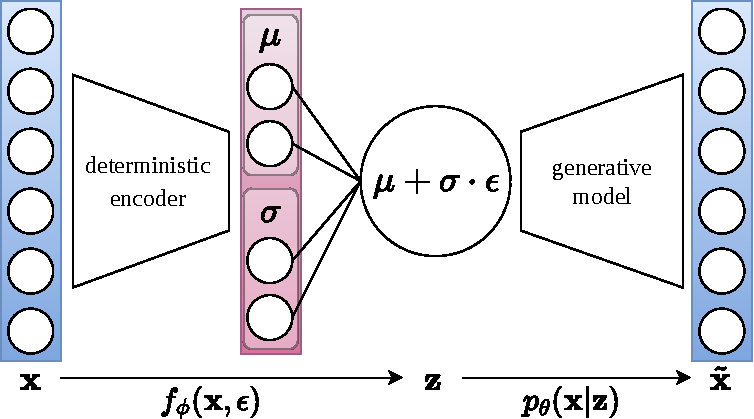
\includegraphics[width=9cm]{rc/vae-reparameterization}
    \end{figure}
    
  \end{frame}

  \begin{frame}{Let's code! (2)}

    \centering
    \includegraphics[width=0.5\textwidth]{rc/colab}\\
    \vspace{1cm}
    \includegraphics[width=0.25\textwidth]{rc/jupyter}

    % VAE avec une/plusieurs couches
    % Entraîner sur MNIST avec différents loss (MSE, cross-entropy)
    % Éventuellement convolutif

    % Observer l'espace latent via t-SNE (comparer avec AE)
    
  \end{frame}

  %%%
  \section{Applications}
  %%%

  \begin{frame}{Dimensionality reduction and Feature extraction}

    Autoencoders can extract useful low-dimensional representations from high-dimensional data. They can be used as:
    \pause
    \begin{itemize}
      \item[$\blacktriangleright$]<2-> a pre-processing step for any other ML algorithm (clustering, supervised classification or regression)
      \item[$\blacktriangleright$]<3-> an unsupervised pre-training prodecure for supervised deep neural networks (e.g. stacked AE pre-training)\\
      $\rightarrow$ see \cite{Hinton2006}, \cite{Erhan2010}, \cite{Vincent2010}
    \end{itemize}
    
  \end{frame}

  \begin{frame}{Data compression}
    
    Autoencoders can be used as a compression algorithm:
    \pause
    \begin{itemize}
      \item[$\blacktriangleright$] \textbf{lossy}
      \pause 
      \item[$\blacktriangleright$] \textbf{data-specific}
    \end{itemize}
    \pause
    Not commonly used in practice\dots

  \end{frame}  

  \begin{frame}{Data augmentation}

    The decoder model can be used to \alert{generate new data samples}:
    \pause
    \begin{itemize}
      \item[$\blacktriangleright$] Deterministic AEs: adding noise, interpolating or extrapolating in latent space \cite{Devries2017}
      \pause
      \item[$\blacktriangleright$] Generative models (VAE, GAN)
    \end{itemize}

  \end{frame}

  \begin{frame}{Anomaly detection}
    
    When the input differs from the training distribution (e.g. an outlier), the model will produce a large reconstruction error. This error can be used to \alert{score anomalies} \cite{Malhotra2016}.

    \begin{figure}
      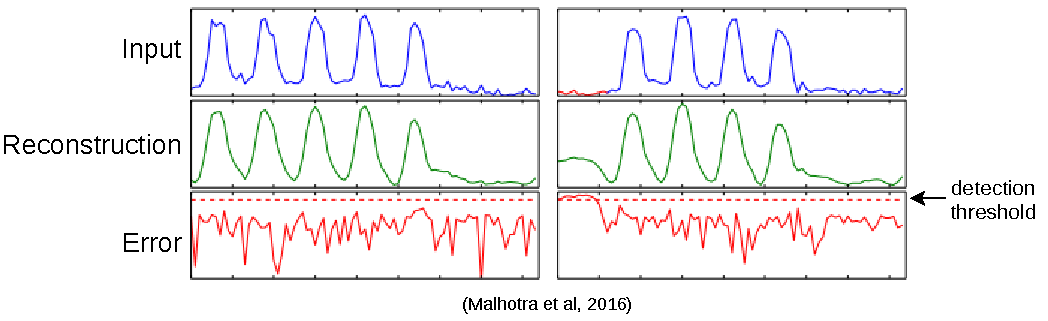
\includegraphics[width=10cm]{rc/anomaly-detection}
    \end{figure}

  \end{frame}

  \begin{frame}[standout]
    Questions?
  \end{frame}

  %%%
  \appendix

  \begin{frame}[allowframebreaks]{References}
    
    \bibliography{references}
    \bibliographystyle{abbrv}
  
  \end{frame}

\end{document}